\section{Durchführung}
\label{sec:Durchfuehrung}
In diesem Kapitel sollen die einzelnen Schritte des Versuches erklärt werden.
Alle Schaltungen werden auf einem Steckbrett, Breadboard oder Steckplatine genannten Konstrukt
aufgebaut. Das vermeidet aufwändiges Löten von Lochrasterplatinen.


\begin{figure}
    \centering
    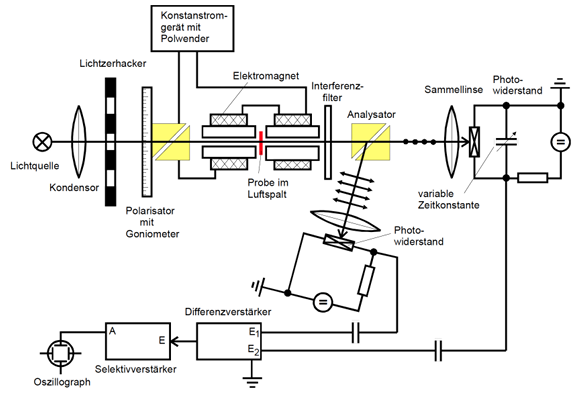
\includegraphics[width=1\textwidth]{content/grafiken/versuchsaufbau.JPG}
    \caption{Der Schematische Versuchsaufbau. [1]}
    \label{fig:versuchsaufbau}
  \end{figure}
